%%%%%%
%%%%%%%%%%%%%%%%%%%%%%%%%%%%%% Title Page Info %%%%%%%%%%%%%%%%%%%%%%%%%%%%%%%%%%%%%%%%%%%
%%%%%%%%%%%%%%%%%%%%%%%%%%%%%%%%%%%%%%%%%%%%%%%%%%%%%%%%%%%%%%%%%%%%%%%%%%%%%%%%%%%%%%%%%%

\documentclass[aspectratio=169,compress]{beamer}
\mode<presentation> 

%\usetheme{Warsaw}
\usetheme{Antibes}
%\usecolortheme{beaver}
\usecolortheme[rgb={0.7,0.0,0.0}]{structure}
%\useoutertheme[subsection=false]{miniframes}

\makeatletter
\setbeamertemplate{headline}
{%
    \begin{beamercolorbox}[wd=\paperwidth,colsep=1.5pt]{upper separation line head}
    \end{beamercolorbox}
    \begin{beamercolorbox}[wd=\paperwidth,ht=2.5ex,dp=1.125ex,%
      leftskip=.3cm,rightskip=.3cm plus1fil]{title in head/foot}
      \usebeamerfont{title in head/foot}\insertshorttitle
    \end{beamercolorbox}
    \begin{beamercolorbox}[wd=\paperwidth,ht=2.5ex,dp=1.125ex,%
      leftskip=.3cm,rightskip=.3cm plus1fil]{section in head/foot}
      \usebeamerfont{section in head/foot}%
      \ifbeamer@tree@showhooks
        \setbox\beamer@tempbox=\hbox{\insertsectionhead}%
        \ifdim\wd\beamer@tempbox>1pt%
          \hskip2pt\raise1.9pt\hbox{\vrule width0.4pt height1.875ex\vrule width 5pt height0.4pt}%
          \hskip1pt%
        \fi%
      \else%  
        \hskip6pt%
      \fi%
      \insertsectionhead
    \end{beamercolorbox}
% Code for subsections removed here
}
\makeatother


% define
% PAra las diapositivas concentradoras de muchos proyectos, no es conveniente la plantilla de puntitos, se debe utilizar otra
%\usepackage{beamerouterthememiniframes} % Para los puntitos 
\setbeamertemplate{footline}[frame number]{}

% include packages
\usepackage{minted}
\usepackage{subfigure}
\usepackage{multicol}
\usepackage{amsmath}
\usepackage{epsfig}
\usepackage{graphicx}
\usepackage[all,knot]{xy}
\usepackage{algorithmic}
\xyoption{arc}
\usepackage{url}
\usepackage{multimedia}
\usepackage{hyperref}
\usepackage{tikz}

\usepackage{pgfpages}
\setbeameroption{hide notes} % Only slides
%\setbeameroption{show only notes} % Only notes
%\setbeameroption{show notes on second screen=right} % Both

\title{Proyectos Dirigidos}
%\title{Proyectos selectos de visión por computadora y aprendizaje automático del Laboratorio de Sistemas Inteligentes de la UPV} % TecMTY
%\title{Recopilación de 10 años de investigación del Laboratorio de Sistemas Inteligentes de la UPV}

\author{Dr. Marco Aurelio Nu\~no Maganda}
\institute{Universidad Politécnica de Victoria\\ Laboratorio de Sistemas Inteligentes \\
mnunom@upv.edu.mx  \vspace{.25cm} }

\date{Octubre 2022}
%\textbf{nmaganda@ccc.inaoep.mx}

%%%%%%%%%%%%%%%%%%%%%%%%%%%%%%%%%%%%%%%%%%%%%%%%%%%%%%%%%%%%%%%%%%%%%%%%%%%%%%%%%%%%%%%%%%
%%%%%%%%%%%%%%%%%%%%%%%%%%%%%% Begin Your Document %%%%%%%%%%%%%%%%%%%%%%%%%%%%%%%%%%%%%%%
%%%%%%%%%%%%%%%%%%%%%%%%%%%%%%%%%%%%%%%%%%%%%%%%%%%%%%%%%%%%%%%%%%%%%%%%%%%%%%%%%%%%%%%%%%

 

%\usepackage[backend=biber,maxcitenames=50,maxbibnames=50,sorting=ydmdddnt]{biblatex}
\usepackage[backend=biber,maxcitenames=50,maxbibnames=50,sorting=none]{biblatex}






%\renewrobustcmd{\mkbibfootnote}{\normalsize\footnotemark\footnotetext}
\setbeamerfont{footnote}{size=\tiny}






\newcommand{\ArchivoPrincipal}{Todos}
\newcommand{\ArchivoSecundario}{Bibliografia}


%Append keywords to identify different bibliography entries.
\DeclareSourcemap{
  \maps[datatype=bibtex, overwrite]{
    \map{
      \perdatasource{\ArchivoPrincipal.bib}
      \step[fieldset=KEYWORDS, fieldvalue=primary, append]
    }
    \map{
      \perdatasource{\ArchivoSecundario.bib}
      \step[fieldset=KEYWORDS, fieldvalue=secundary, append]
    }    
  }
}


\addbibresource{\ArchivoPrincipal.bib}
\addbibresource{\ArchivoSecundario.bib}

\usepackage{listings}
 
 \AtBeginSection[]
{
    \begin{frame}
        \frametitle{Outline}
        \tableofcontents[currentsection]
    \end{frame}
}

\makeatletter
\def\@makefnmark{}
\makeatletter
\setbeamertemplate{footnote}{%
  \parindent 1em\noindent
  \raggedright
  *  
  \insertfootnotetext\par
}


\newcommand{\EntradaBibtex}{InvalidEntry}

\begin{document}










\section{2002_ArquitecturaPiramide}
\frame
{
\frametitle{\citetitle{MarcoNunoTesisLicenciatura_2002}}
\begin{columns}
    \column {0.4\textwidth}
\begin{itemize}    
\item Proyecto de asignatura de maestría: Implementación de la Pirámide en la tarjeta RC100 de Celoxica. 
\item Entrada: Video en RCA, Salida a monitor VGA.
\end{itemize}
    \column {0.3\textwidth}
\begin{center}
    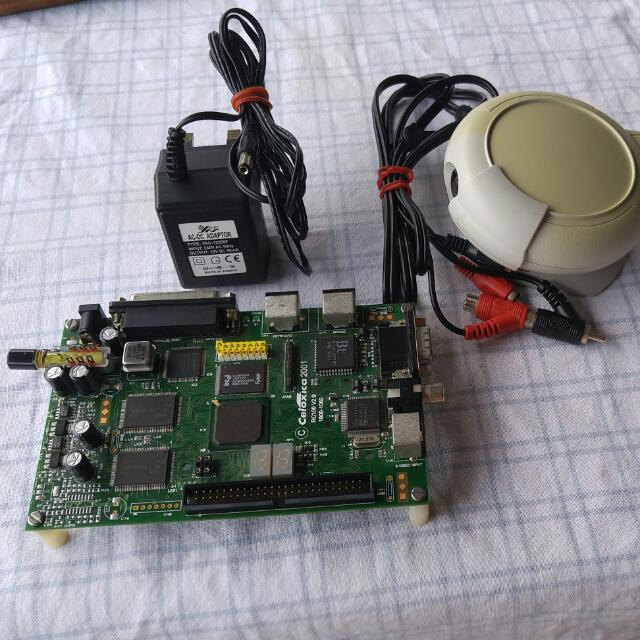
\includegraphics[width=0.9\textwidth]{Figs/celoxica_2001_rc100}
\end{center}    

    \column {0.3\textwidth} 
    \begin{center}
    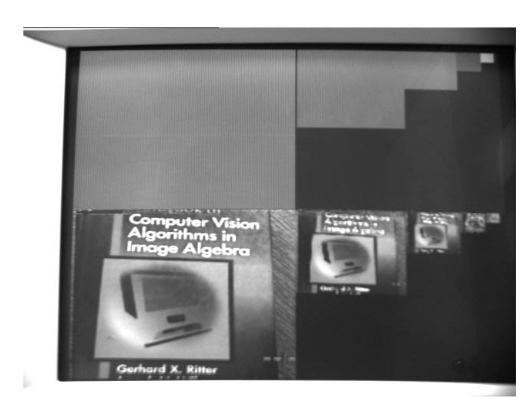
\includegraphics[width=0.9\textwidth]{Figs/2002_PiramideMonitor_RC100}\\
        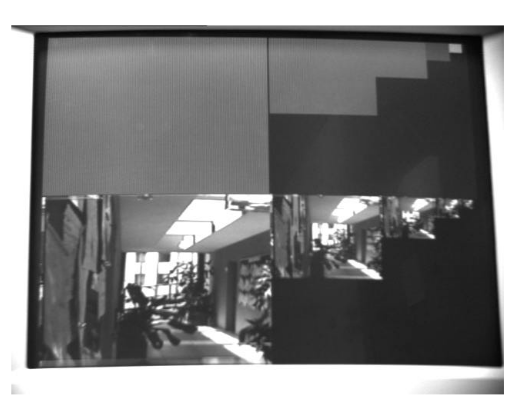
\includegraphics[width=0.9\textwidth]{Figs/2002_PiramideMonitor_RC100_2}
            \end{center}
\end{columns}     

\footnotetext[1]{\fullcite{MarcoNunoTesisLicenciatura_2002}}
}

\frame{
\frametitle{Arquitectura Propuesta}
\begin{columns}
    \column {0.5\textwidth}
 \begin{itemize} 
\item Procesamiento de video en tiempo real.
\item Procesamiento simultaneo (doble búffer): Un proceso almacenaba un frame de memoria, mientras que otro procesaba el frame previamente almacenado.
\item Lenguaje: Handel-C (RIP).
\item DK1 Design Suite.
\item FPGA: Spartan-II.
\item Tarjeta: RC-100 de Celoxica.
    
\end{itemize}
    
    \column {0.5\textwidth} 
    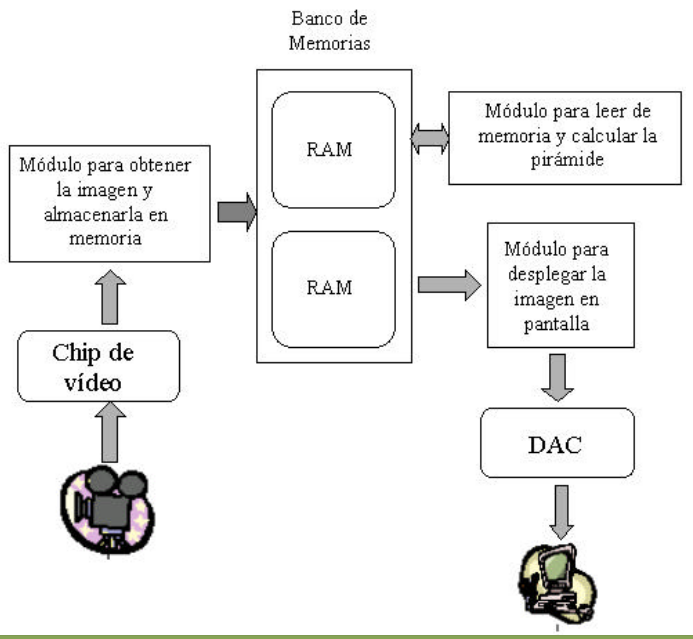
\includegraphics[width=0.9\textwidth]{Figs/2002_PiramideMonitor_RC100_Arquitectura_3}
\end{columns}     
}


\section{2003_PiramideMultiresolucion}

\frame
{
\frametitle{\citetitle{MarcoNuno_CongArbIng_2003_12_00}}
\begin{columns}
  \column {0.5\textwidth}  
En ese artículo se reportan dos arquitecturas hardware:
\begin{itemize}
\item Estimación de la pirámide de imágenes
\item Calcular la correlación entre dos imágenes
\end{itemize}
Tres aplicaciones:
\begin{itemize}
\item Seguimiento.
\item Estabilización.
\item Generación de mosaicos.
\end{itemize}
  \column {0.5\textwidth}  
  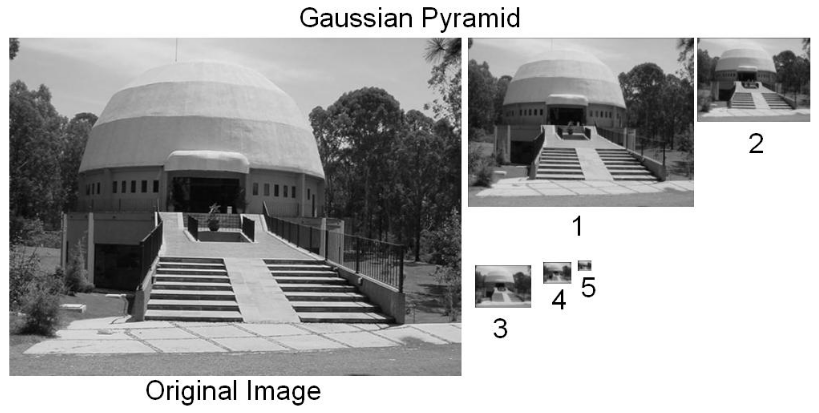
\includegraphics[width=0.9\textwidth]{Figs/Piramide}
  \end{columns}
\footnotetext[1]{\fullcite{MarcoNuno_CongArbIng_2003_12_00}}
}

\frame{
\frametitle{Seguimiento, Estabilización y Mosaicos}
\begin{columns}
    \column {0.5\textwidth}
    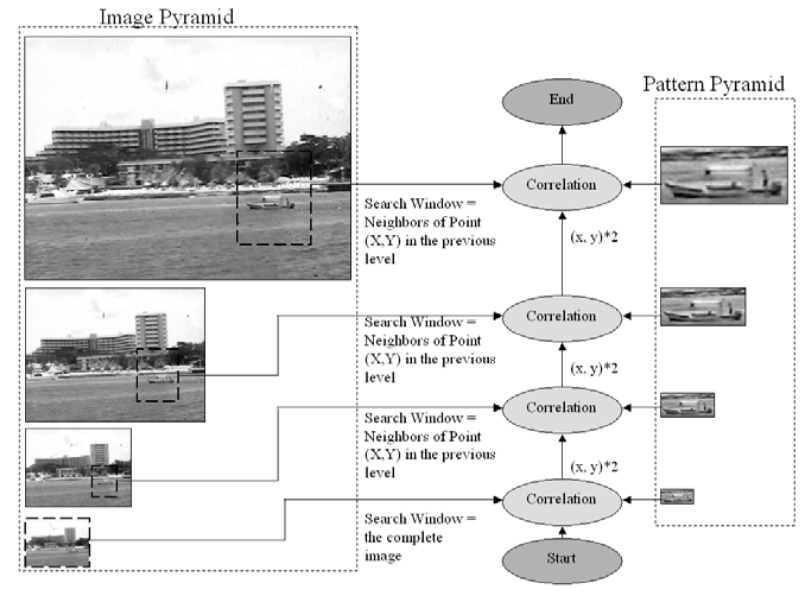
\includegraphics[width=0.9\textwidth]{Figs/Piramide_Correlacion}
    \column {0.5\textwidth}    
        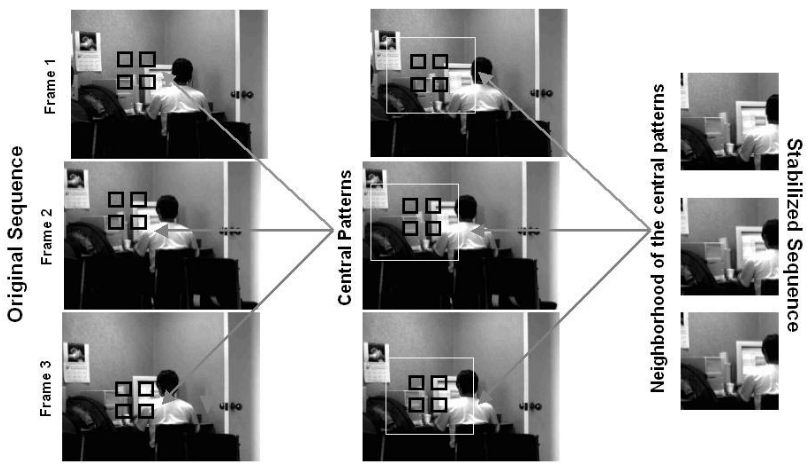
\includegraphics[width=0.8\textwidth]{Figs/Piramide_Estabilizacion}\\
        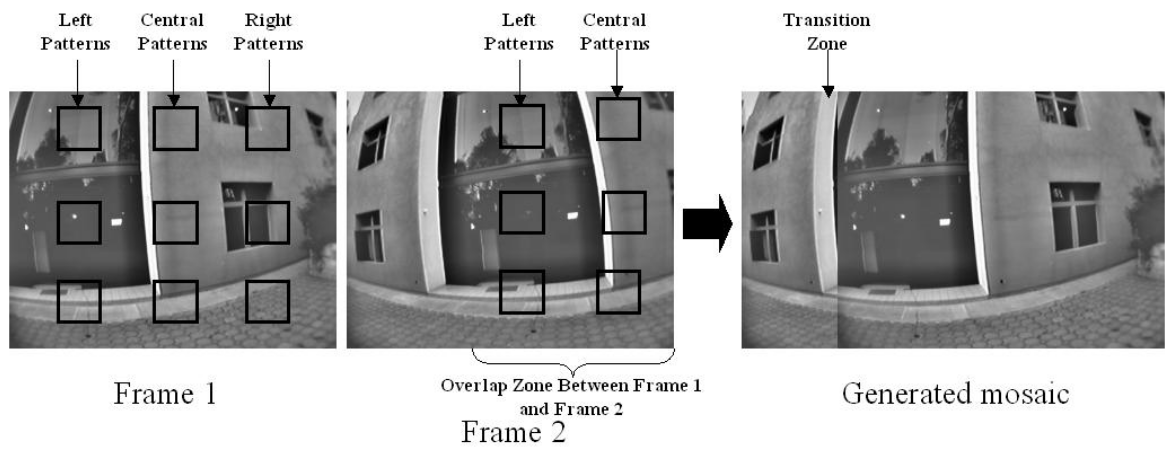
\includegraphics[width=0.98\textwidth]{Figs/Piramide_Mosaicos}
      
\end{columns}    
}

\frame{
\frametitle{Resultados}
    \begin{columns}
        \column {0.5\textwidth}
            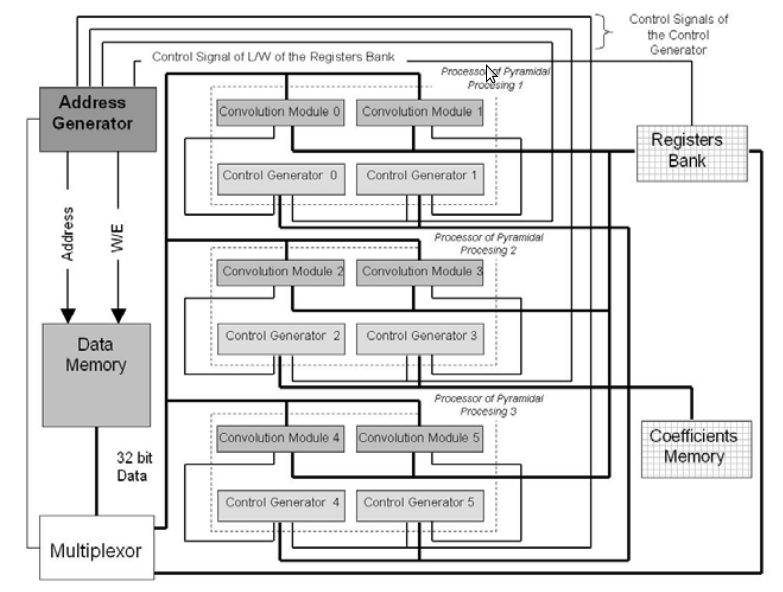
\includegraphics[width=0.8\textwidth]{Figs/Piramide_Arquitectura1}
        \column {0.5\textwidth}    
            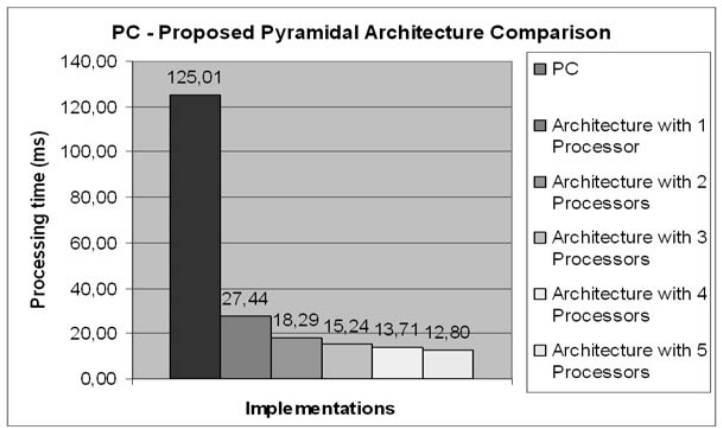
\includegraphics[width=0.9\textwidth]{Figs/Piramide_GraficaComparacion}
    \end{columns}    
}


\end{document}
